\documentclass[14pt]{article}

\usepackage[utf8x]{inputenc}
\usepackage[russian]{babel}
\usepackage{graphicx}
\graphicspath{{images/}}
\DeclareGraphicsExtensions{.pdf,.png,.jpg}

\usepackage{amsmath}
\usepackage{pgfplots}

\usepackage{geometry} % Меняем поля страницы
\geometry{left=2cm}% левое поле
\geometry{right=1.5cm}% правое поле
\geometry{top=2cm}% верхнее поле
\geometry{bottom=2cm}% нижнее поле

\renewcommand{\theenumi}{\arabic{enumi}}
\renewcommand{\labelenumi}{\arabic{enumi}}
\renewcommand{\theenumii}{.\arabic{enumii}}
\renewcommand{\labelenumii}{\arabic{enumi}.\arabic{enumii}.}
\renewcommand{\theenumiii}{.\arabic{enumiii}}
\renewcommand{\labelenumiii}{\arabic{enumi}.\arabic{enumii}.\arabic{enumiii}.}

\begin{document}
\begin{titlepage}
	\begin{center}
		\fontsize{18pt}{20pt}\selectfont
		\textbf{Работа 4.3.6.}	
	
		\vspace{5cm}
		\fontsize{24pt}{25pt}\selectfont
		Саморепродукция
	\end{center}
	\begin{flushright}
		\fontsize{18pt}{20pt}\selectfont
		\vspace{14cm}
		\hspace{-3cm}
		\textit{Корнеев Е.С.}
	\end{flushright}		
\end{titlepage}

\begin{center}
	\fontsize{16pt}{18pt}\selectfont	
	Саморепродукция
\end{center}


\fontsize{14pt}{16pt}\selectfont
\vspace{1cm}
\textbf{Цель работы:} Изучение явления саморепродукции и применение его к измерению параметров периодических структур.

\vspace{1cm}
\textbf{Оборудование:} лазер, кассета с сетками, мира, короткофокусная
линза с микрометрическим винтом, экран, линейка.

\vspace{1cm}

При дифракции на предмете с периодической структурой наблюдается
интересное явление: на некотором расстоянии от предмета
вдоль направления распространения волны появляется изображение,
которое потом периодически повторяется — \textsl{репродуцируется}.


Этот эффект имеет простое физическое объяснение. Если на
пути распространения плоской волны в плоскости $z = 0$ расположить
транспарант (например, изображение предмета на фотоплёнке
или стеклянной пластинке) с функцией пропускания, отличной
от константы, то на выходе из него в плоскости $z = 0_+$
волна уже перестанет быть плоской. Если при этом функция пропускания
транспаранта -- периодическая функция координат, периодической
функцией будет и комплексная амплитуда волны на
выходе из транспаранта, т. е. в плоскости $z = 0_+$. Периодическому
распределению комплексной амплитуды в плоскости $z = 0_+$
будет соответствовать дискретный набор плоских волн с кратными
пространственными частотами. При этом оказывается, что существуют
плоскости (при $z > 0$), где все плоские волны имеют
те же самые фазовые соотношения, что и в плоскости $z = 0_+$.
В результате интерференции этих волн получается изображение,
тождественное исходному периодическому объекту.


Найдём выражение для расстояния между этими плоскостями.
Напомним, что плоской монохроматической волной называется
волна вида
\begin{equation}
	E(\vec{r}, t) = a_0e^{-i(\omega t - \vec{k}\vec{r} - \psi_0)}
\end{equation}
\noindent где амплитуда $a_0$ -- действительная постоянная, $\omega$ -- круговая частота,
$\vec{k}$ -- волновой вектор $(|\vec{k}| = 2\pi/\lambda)$, $\psi_0$ -- начальная фаза.
Колебания происходят синфазно во всех точках плоскости:
\begin{equation}
	\vec{k}\vec{r} = ux + vy + \sqrt{k^2 - u^2 - v^2}\cdot z = const
\end{equation}

Направление распространения плоской монохроматической волны
характеризуется волновым вектором
$\vec{k}$, а $u$ и $v$ есть проекции его на оси координат $x$ и $y$ соответственно.
В дальнейшем мы будем опускать зависимость от времени $e^{−i\omega t}$ и использовать для
описания монохроматической волны комплексную амплитуду. Для плоской волны (1)
комплексную амплитуду можно представить в виде
\begin{equation}
	f(x,y,z) = a_0e^{i\psi_0}e^{i(ux + vy)}e^{i\sqrt{k^2 - u^2 - v^2}z} = f(x,y,0)\cdot e^{i\sqrt{k^2 - u^2 - v^2}z}
\end{equation}
\noindent Таким образом, для того чтобы получить комплексную амплитуду
плоской волны в произвольной плоскости $z = const$, надо ее значение в плоскости $z = 0$ домножить на фазовый множитель
$e^{i\sqrt{k^2 - u^2 - v^2}z}$.

Пусть плоская волна падает перпендикулярно на транспарант, расположенный в плоскости
$z = 0$, тогда для падающей волны $u = v = 0$, и комплексная амплитуда волны на входе в транспарант
является константой $a_0e^{i\psi_0}$. Комплексную амплитуду волны в плоскости $z = 0_+$ на выходе из транспаранта получаем, умножив
комплексную амплитуду на входе в транспарант на функцию пропускания транспаранта $t(x,y)$. Это правило является определением
понятия \textsl{функции пропускания транспаранта}. Если функция пропускания периодическая с периодом $d$ (для простоты рассмотрим
одномерный случай $t(x,y) = t(x)$), то комплексная амплитуда на выходе из транспаранта $a_0e^{i\psi_0}t(x)$ также периодическая функция с тем
же периодом $d$. Согласно теореме Фурье (доказываемой в курсе математического анализа) периодическая функция
$a_0e^{i\psi_0}t(x)$ может быть представлена в виде ряда Фурье -- суммы гармонических составляющих с кратными пространственными частотами
$u_n = 2\pi n/d$:
$$
	f(x, 0_+) = a_0e^{i\psi_0}t(x) = a_0 + \sum_{n = 1}^\infty [a_n\cos(nu_nx) + b_n\sin(nu_nx)]
$$
\noindent или в комплексной форме --
\begin{equation}
	f(x, 0_+) = \sum_{n = -\infty}^\infty c_ne^{iu_nx} = \sum_{n = -\infty}^\infty c_ne^{i\frac{2\pi}{d}nx}
\end{equation}
\noindent Опираясь на теорему единственности решения волнового уравнения при заданных граничных условиях, мы можем утверждать,
что периодическому распределению комплексной амплитуды в плоскости $z = 0_+$ будет соответствовать при $z > 0$ дискретный набор
плоских волн с кратными пространственными частотами $u_n$. Как видно из (3), для плоской волны с пространственной частотой
$u_n$ волновой вектор $\vec{k}$ имеет проекции $u_n, 0, \sqrt{k^2 - u_n^2}$. Разложение волны, продифрагировавшей на транспаранте,
в ряд по плоским волнам позволяет легко найти комплексную амплитуду волны в произвольной плоскости $z = const$. Для этого достаточно домножить
комплексные амплитуды плоских волн в суперпозиции (4) на соответствующий фазовый множитель $exp(i\sqrt{k^2 - u_n^2})$:
\begin{equation}
	f(x,z) = \sum_{n = -\infty}^{\infty} c_ne^{iu_nx}e^{i\sqrt{k^2-u_n^2}z}
\end{equation}

Каждая плоская волна в суперпозиции (4) приобрела при распространении от транспаранта до плоскости наблюдения
$z = const$ набег фазы:
$$
	\varphi_n = \sqrt{k^2-u_n^2}\cdot z
$$

Для параксиальных волн $(u_n \ll 1)$:
\begin{equation}
	\varphi_n \approx kz - \frac{u_n^2}{2k}z
\end{equation}
\noindent и, таким образом, разность набегов фазы для любых двух плоских волн (с индексом $n$ и $m$) равна
\begin{equation}
	\Delta\varphi_{n,m} = (u_m^2 - u_n^2)\frac{z}{2k} = (m^2 - n^2)\frac{\pi\lambda}{d^2}z
\end{equation}

\begin{figure}[h!]
	\center{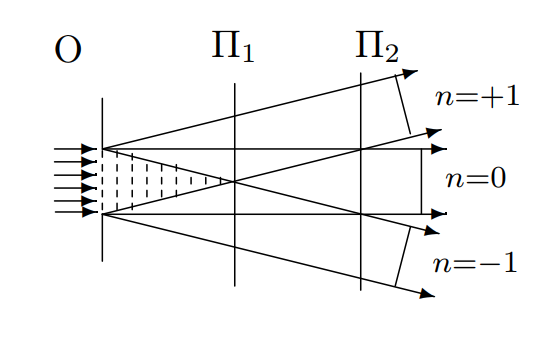
\includegraphics[width = 8cm]{1}}
	\caption{Принципиальная схема дифракции на сетке. Между сеткой 0 и плоскостью $\Pi_1$ наблюдаются репродуцированные изображения сетки}
	\label{fig:image}
\end{figure}

\noindent Легко видеть, что в плоскости наблюдения $z_0 = 2d^2/\lambda$ разность фазовых набегов оказывается кратной $2\pi$ для любых гармоник,
входящих в состав суперпозиции (4), т.е. совпадают фазовые соотношения между колебаниями, которые создаются всеми плоскими волнами, входящими
в состав суперпозиции (4) в предметной плоскости $z = 0_+$ в плоскости изображения $z_1 = 2d^2/\lambda$. Поэтому в результате интерференции этих волн мы получаем изображение, тождественное исходному периодическому объекту. Описанное явление называется \textsl{эффектом саморепродукции}. Световая волна сама (без каких-либо 
линз или зеркал) создает изображение исходного объекта. Ясно, что все сказанное справедливо и для любого расстояния $z_N$, кратного $z_1$:
\begin{equation}
	z_N = \frac{2d^2}{\lambda}N
\end{equation}

На опыте, вследствие ограниченности поперечного сечения светового пучка лазера, наблюдаются только несколько репродуцированных изображений решетки. Поясним этот эффект с помощью рис. 1.

На нем изображены только три продифрагировавших луча соответственно нулевого $(n = 0)$ и $\pm$ первого порядка $(n = \pm1)$. Там, где эти лучи перекрываются, образуется интерференционная картина с периодом, как раз равным периоду решетки $d$. Спроектировав картину с помощью линзы на экран, мы увидим изображения синусоидальной решетки
с плавным переходом от максимумов к минимумам. Для того чтобы наблюдать более тонкие детали, необходимо, чтобы в плоскости наблюдения перекрывались лучи более высоких дифракционных порядков. На краях, где перекрываются только два луча ($n = 0$ и $n = +1$ или $n = 0$ и $n = −1$), также образуется интерференционная картина с периодом
$d$, но менее контрастная.

Таким образом, левее плоскости $\Pi_1$ мы будем наблюдать, хотя и слегка размытые, репродуцированные изображения решетки. Правее плоскости $\Pi_2$ репродуцированных изображений не будет.

\vspace{1cm}
\textbf{Экспериментальная установка.} Хорошим приближением к плоской волне в нашем эксперименте является излучение лазера. Луч лазера падает перпендикулярно на периодический объект $O$, установленный в плоскости $P_0$ (рис. 2). 

За плоскостью $P_0$ (в плоскостях $P_1$ -- $P_N$ ) периодически по $z$ возникают изображения объекта, которые с помощью линзы Л можно поочерёдно проецировать на экран,
установленный в плоскости Э. Если убрать линзу, то на экране наблюдается картина дифракции луча лазера на периодическом объекте.

\begin{figure}[h!]
	\center{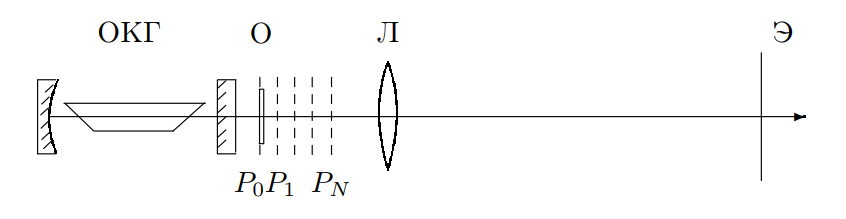
\includegraphics[width = 15cm]{2}}
	\caption{Схема установки: ОКГ -- гелий-неоновый лазер, 0 -- двумерная решетка, $P_N$ -- плоскости, где наблюдаются репродуцированные изображения, Л -- короткофокусная 	линза, Э -- экран для наблюдения изображения объекта}
	\label{fig:image}
\end{figure}

Экран устанавливается достаточно далеко от объекта, так что продифрагировавшие лучи, соответствующие различным порядкам дифракции ($\sin\varphi_n = n\lambda/d$), разделяются.


Измерив расстояние между дифракционными максимумами и расстояние от объекта до экрана, мы определим $\sin\varphi_n$ и $d$.


В нашей работе в к ачестве периодических объектов применяется мира -- набор различным образом ориентированных одномерных решеток разного периода (рис. 4), а также двумерная решетка-сетка. Сетку можно рассматривать как две взаимно перпендикулярные решетки. Узкий пучок монохроматического света, пройдя через первую решетку с вертикальными штрихами, должен дать совокупность максимумов, расположенных вдоль горизонтальной линии.

Световой пучок, соответствующий каждому максимуму, проходя через вторую решетку, распадается на новую совокупность пучков, дающих максимумы вдоль вертикальной линии.
В результате главные максимумы возникают тогда, когда одновременно выполняются условия
\begin{equation}
	d\sin\varphi_x = n_x\lambda,~~d\sin\varphi_y = n_y\lambda
\end{equation}
\noindent где $n_x$ и $n_y$ -- два целых числа, характеризующих порядки дифракционных максимумов, $\varphi_x$ и $\varphi_y$ -- направления на главные дифракционные
максимумы в горизонтальной и вертикальной плоскостях соответственно (рис. 3). Максимумы показаны кружками, размеры которых характеризуют интенсивность.

\begin{figure}[h!]
	\center{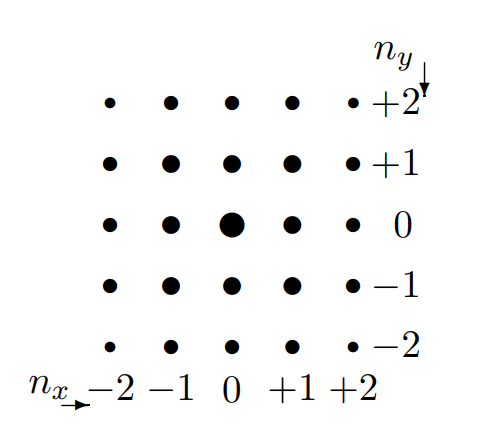
\includegraphics[width = 7cm]{3}}
	\caption{Спектр решётки-сетки}
	\label{fig:image}
\end{figure}



\end{document}